\chapter{Functional Analysis}
The first step in determining the requirements for the aircraft is looking at its function in detail. This can be done using a functional flow diagram (FFD), which analyses a typical mission of the aircraft. From that, key functions can be identified and later formatted as a functional breakdown structure (FBS). The two diagrams are available as  A3 PDF pages at the end of this chapter.

\section{Mission Profile}
Based on the requirements stated in \autoref{tab:system_requirements}, it was decided that the mission profile will consist of the general phases that are stated in \cite{Vos}. A diagram of the mission profile can be found in \autoref{fig:mission_profile}

\begin{figure}[H]
    \centering
    
\includegraphics[width=\linewidth]{figures/Mission Profil.png}
    \caption{General Mission Profile}
    \label{fig:mission_profile}
\end{figure}

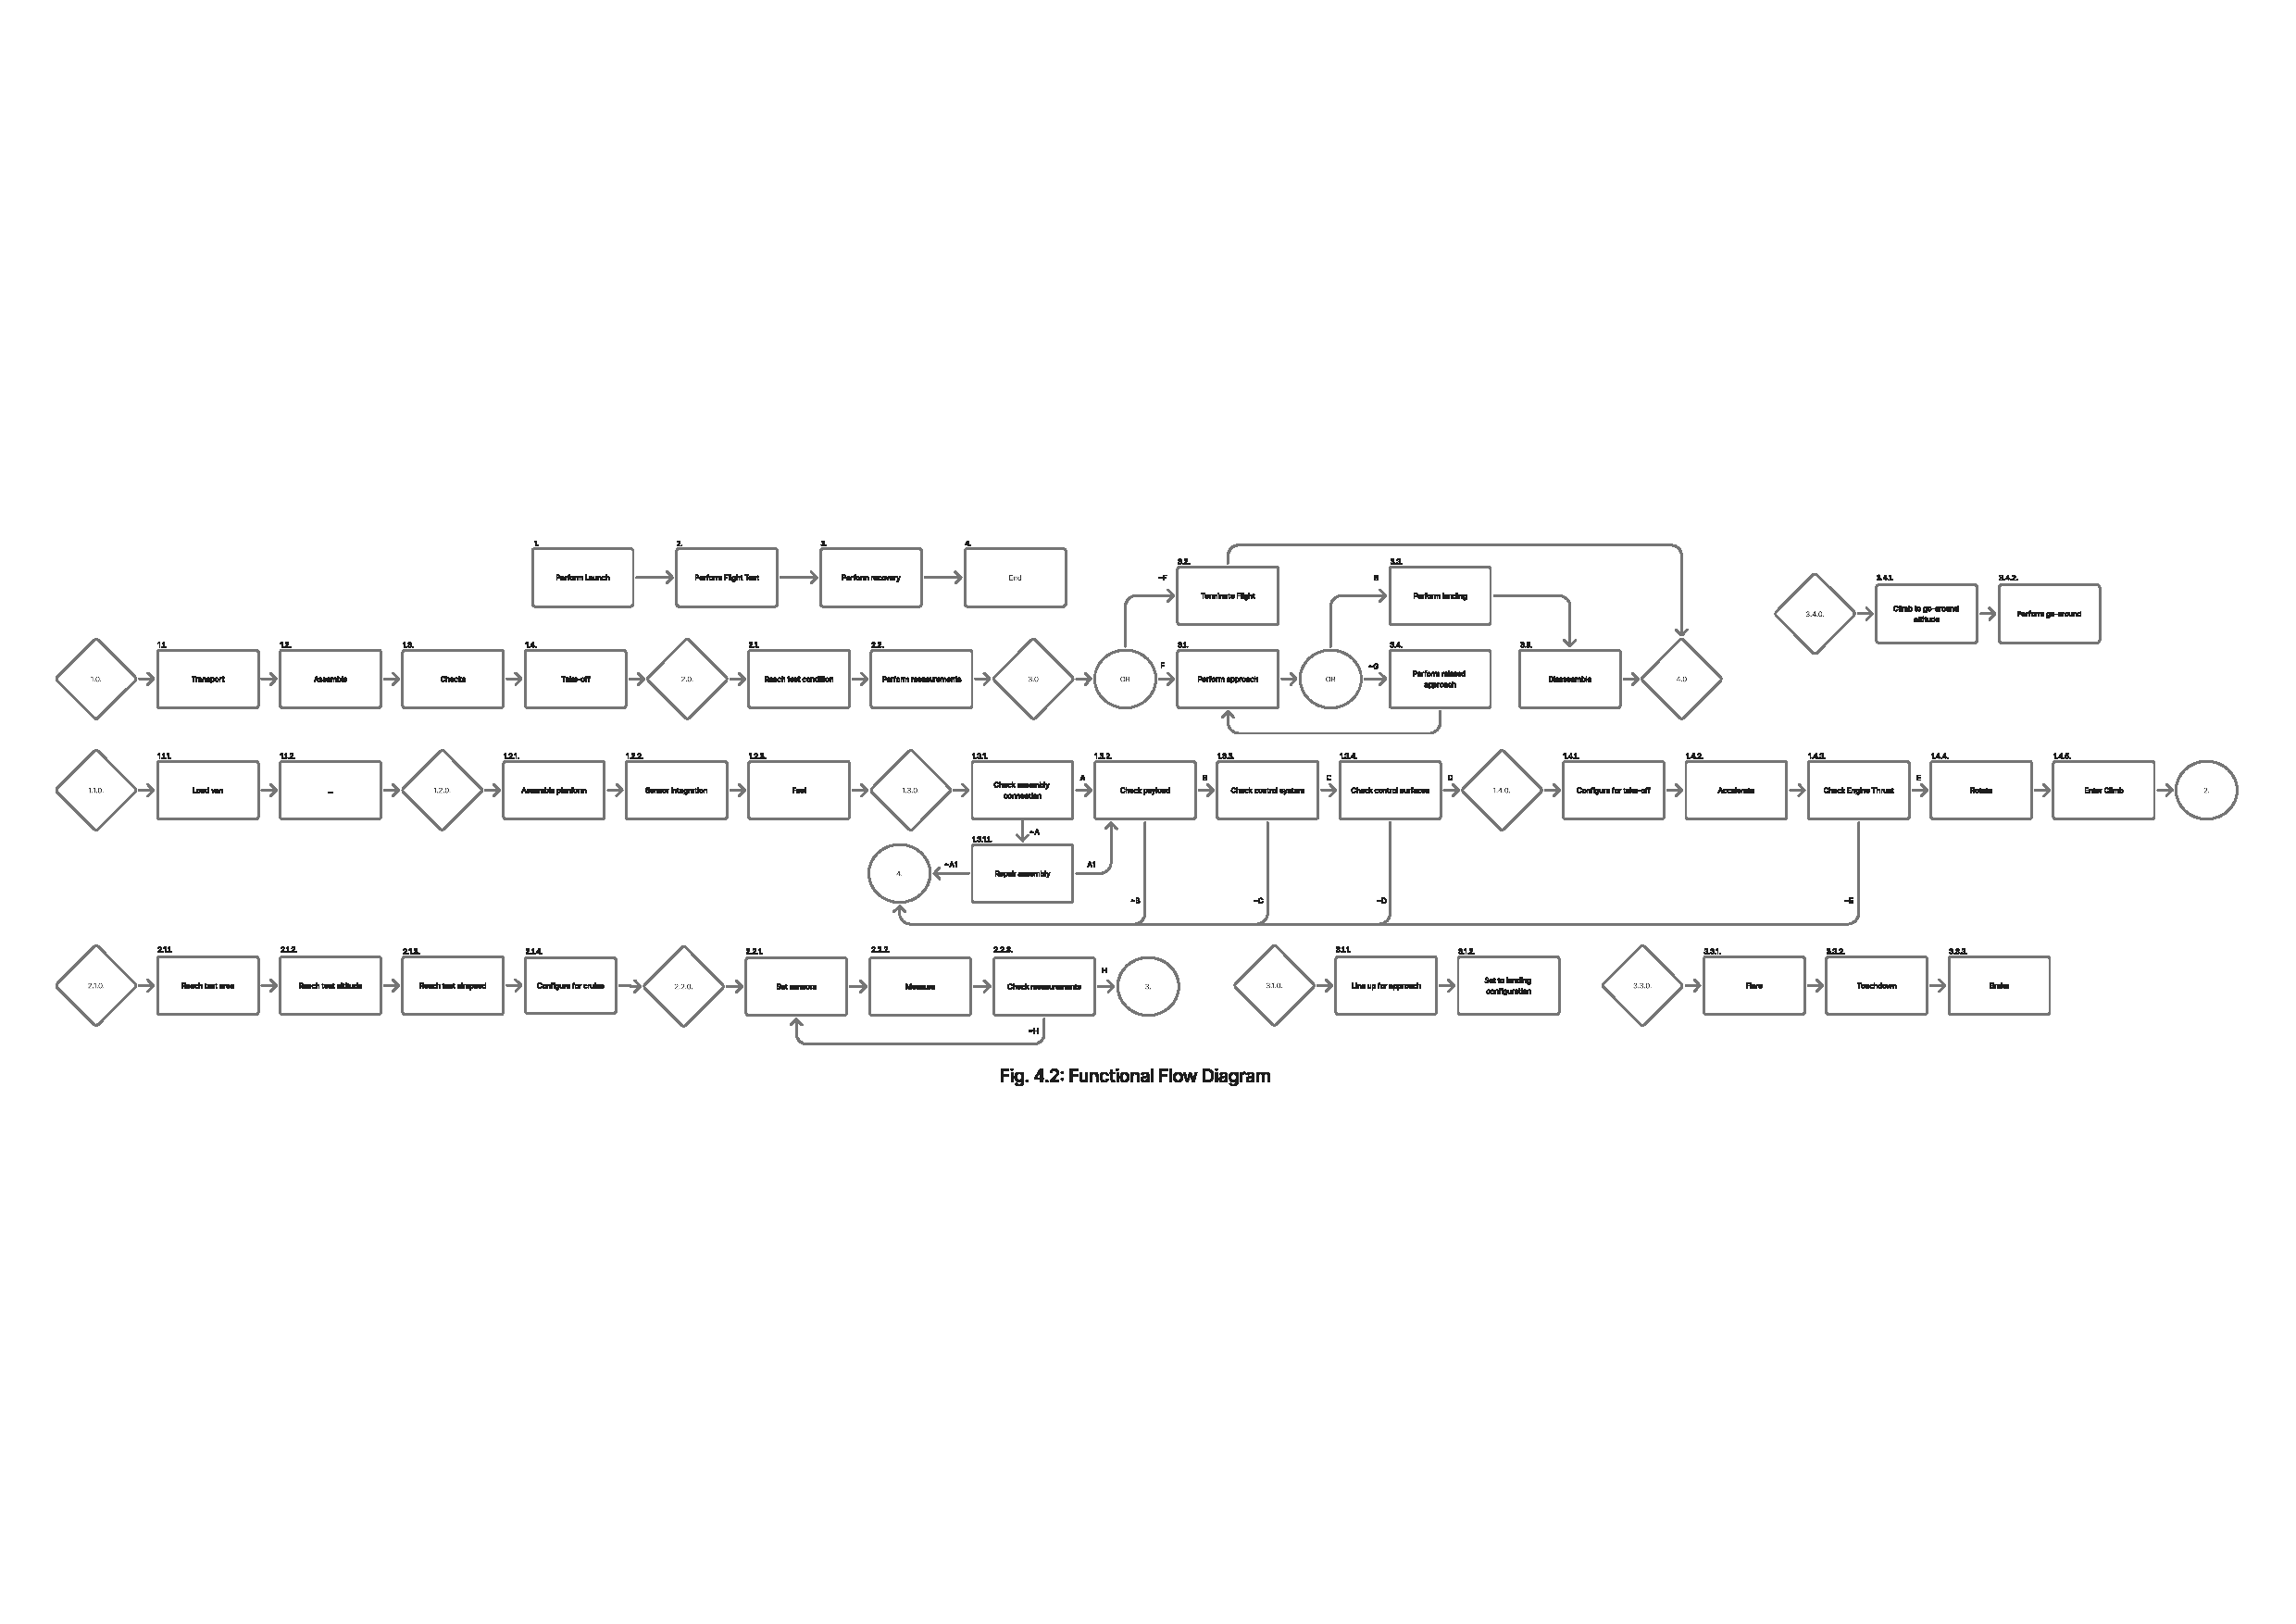
\includepdf[pages=-,fitpaper=true, width=420mm, keepaspectratio]{figures/Functional Flow Diagram.pdf}


\includepdf[pages=-,fitpaper=true, width=420mm, keepaspectratio]{figures/Functional Breakdown Structure.pdf}